\subsection{Abstract Syntax of \bcool}
\begin{figure}
	\center
	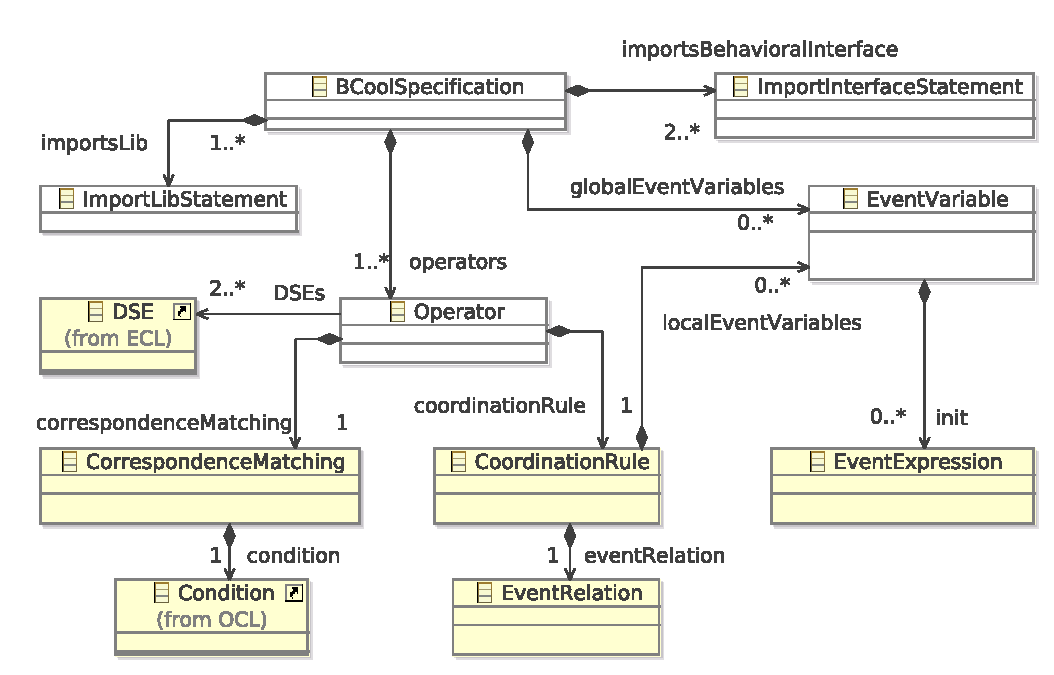
\includegraphics[width=.8\textwidth]{bcool/figs/BcoolMM}
	\caption{Simplified View of \bcool Abstract Syntax}
	\label{fig:bcool}
\end{figure}

The abstract syntax of \bcool is defined by its metamodel (see Figure~\ref{fig:bcool}). The root element is a \emph{BCoolSpecification} that contains \emph{Operators}. Each operator refers to \dse to specify what event types it coordinates. To get the \dse, a \bcool specification imports language behavioral interfaces (\emph{importsInterfaceStatements}). The number of imported interfaces is related with the number of models that the specification accepts as input. Since the \bcool specification is applied at least between two models, it imports at least two interfaces. The same interface can be imported several times to allow the specification of operators between homogeneous languages.   

To build the running example operator, we need to synchronize FSMEvents and Actions. This is done by coordinating instances of \dse \emph{occurs} and instances of \dse \emph{executeIt}. To specify this in \bcool, we first define a specification named \emph{TFSMAndActivity} and we import the language behavioral interface of each language, named \emph{activity} and \emph{tfsm} (Listing~\ref{lst:bcoolrunningexample}: line 3 and 4). Then, the operator \emph{SyncFSMEventsAndActions} is defined, which refers to the \dse \emph{occurs} and \emph{executeIt}, mapped as \emph{FSMEventOccurs} and \emph{ActionExecute} respectively (Listing~\ref{lst:bcoolrunningexample}: line 5). 
	
	 
	\begin{lstlisting}[language=bcool,
	caption={\bcool specification of the running example operator between the TFSM and Activity languages},
	label={lst:bcoolrunningexample}, 
	basicstyle=\scriptsize\ttfamily, backgroundcolor=\color{LGrey}, numbers=left, xleftmargin=2pt]
	BCOoLSpec TFSMAndActivity
	ImportLib "facilities.moccml"
	ImportInterface "activitySemantics.ecl" as activity
	ImportInterface "TFSM.ecl" as tfsm
	Operator SyncFSMEventsAndActions(ActionExecute:activity::executeIt, FSMEventOccurs:tfsm::occurs)
	when (ActionExecute.name = FSMEventOccurs.name);
	do   RendezVous(ActionExecute, FSMEventOccurs)
	end operator
	\end{lstlisting}
	
In \bcool, operators are used to specify when and how instances of the referred \dse must be coordinated. To do so, each operator contains a \emph{correspondence matching} and a \emph{coordination rule}. The former is used to select instance of \dse and the latter to express how the selected instances must be coordinated. 
	
A \emph{correspondence matching} selects instances of \dse by using a \emph{Condition} that contains an OCL Boolean expression. To express the boolean expression, the context of the \dse can be queried to get a specific syntactic element, \eg attribute \emph{name}. The boolean condition is thus used to compare the queried elements. The correspondence matching acts as a precondition for the coordination rule, \ie it is a predicate that defines when the coordination rule must be applied to the given instances of \dse. For instance, for the running example, we query the context of the \dse to get the attribute \emph{name} (Listing~\ref{lst:bcoolrunningexample}: line 6). Then, the attributes are used as operands for the boolean condition. When an instance of \dse \emph{occurs} and an instance of \dse \emph{executeIt} have the same name, the pairs are selected and the coordination rule is applied.
	
The \emph{coordination rule} specifies how the selected instances of \dse must be coordinated. To do so, it contains an \emph{EventRelation} and possibly some \emph{EventVariables} (\emph{localEventVariables}).    	
	
The event relation is used to restrict the relative order of the occurrences of events used as parameters. Its actual parameters can be instances of \dse, some \emph{EventVariables} and/or constants (\eg integer constants). For example, the running example operator must specify a strong synchronization between the events. To express that, we use the event relation \emph{Rendezvous} between the selected instances of \dse \emph{occurs} and \emph{executeIt} (Listing~\ref{lst:bcoolrunningexample}: line 7). This relation accepts two events as arguments and forces the occurrences of these events to happen simultaneously. To illustrate this, Figure~\ref{fig:runningrdv} partially shows the resulting coordination when the running example operator is used to coordinate the models of the coffee machine. In the figure, the occurrences of the \mse \emph{selectCoffee:occurs} and \emph{selectCoffee:executeIt} are forced to happen simultaneously.   
	
	\begin{figure}[h]
		\center
		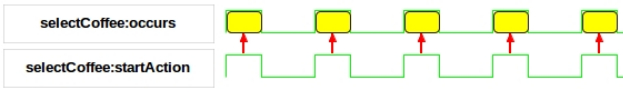
\includegraphics[width=.8\textwidth]{bcool/figs/runningrdv}
		\caption{Resulting coordination of the Coffee Machine by using the event relation Rendezvous}
		\label{fig:runningrdv}
	\end{figure}


Conjointly with an event relation, \bcool enables the definition of \emph{EventVariables} to express more complex coordination rules. An event variable can be either defined locally within the coordination rule (\emph{localEventVariables}) or globally for the whole specification (\emph{globalEventVariables}). These variables either define global events used across different operators, or create a new event from the selected instances of \dse and possibly from attributes of the input models. The definition of these events is made by using an \emph{EventExpression}. An event expression returns a new event from given parameters. For instance, this can be used to select only some occurrences of a \dse instance, thus allowing the implementation of filters. An event expression can also be used to join in a single event the occurrences of different events (union). When used in the coordination rule, the resulting events can be used as parameters of event relations, constraining by transitivity (some of) the occurrences of \dse instances.

To illustrate the use of event variables, we suppose the situation in which the coordination between events relies on a global synchronization clock. This is often the case in synchronous digital systems in which a clock signal is used to coordinate the actions in a circuit. Thus, we slightly modify the running example operator by considering the case in which the coordination between instances of \dse \emph{occurs} and instances of \dse \emph{executeIt} relies on a global clock signal. The selected instances of \dse \emph{occurs} (the \emph{sampledEvent}) are sampled by a global clock (the \emph{trigger}). This results in a new event that ticks always in coincidence with the \emph{trigger}. Each of its occurrences represents the last occurrence of the \emph{sampledEvent} sampled by the \emph{trigger}. 
	
\begin{lstlisting}[language=bcool,
caption={\bcool specification of an operator that illustrates the use of Event Variables},
label={lst:bcoolrunningexampletimed}, 
basicstyle=\scriptsize\ttfamily, backgroundcolor=\color{LGrey}, numbers=left, xleftmargin=2pt]
BCOoLSpec TimedTFSMandActivity
ImportLib "facilities.moccml"
ImportInterface "activitySemantics.ecl" as activity
ImportInterface "TFSM.ecl" as tfsm
Global Event globalClock;
Operator SyncFSMEventsAndActions(ActionExecute:activity::executeIt, FSMEventOccurs:tfsm::occurs)
when (dse1.name = dse2.name);
do
	Local Event sampledOccurs = SampledOn (FSMEventOccurs, globalClock);
	RendezVous(ActionExecute, sampledoccurs)
end operator
\end{lstlisting}
			
To specify this in \bcool, we define a new specification named \emph{TimedTFSMandActivity} (Listing~\ref{lst:bcoolrunningexampletimed}). We first define a global event variable named \emph{globalClock} (Listing~\ref{lst:bcoolrunningexampletimed}: line 5). This global event variable represents the global synchronization clock. Then, in the coordination rule, we use the globalClock together with the \dse \emph{occurs} to create a new local event named \emph{sampledOccurs} (Listing~\ref{lst:bcoolrunningexampletimed}: line 9). To initialize this local variable, we use the event expression \emph{SampleOn}. This expression accepts two events as parameters: the \emph{SampledEvent} and the \emph{Trigger}. The expression creates a new event by sampling the \emph{SampledEvent} by the \emph{Trigger} event. This results in a new event that ticks always after the \emph{SampledEvent} and coincides with the occurrences of the \emph{Trigger} event. In our case, we sample the select instances of the \dse \emph{occurs} (\ie \emph{SampledEvent}) by the event global clock (\ie \emph{Trigger}), which results in the local event variable \emph{sampledOccurs}. Then, in the coordination rule, we coordinate the instances of \dse \emph{executeIt} and the resulting local event \emph{sampledOccurs} by a Rendezvous (Listing~\ref{lst:bcoolrunningexampletimed}: line 10). 

To illustrate the resulting coordination, we use this specification to coordinate the models of the coffee machine. Figure~\ref{fig:runningeventvar} shows the partial resulting coordination between the \mse \emph{selectCoffee:occurs} and \emph{selectCoffee:executeIt} when a global clock is used. The occurrences of the event \emph{selectCoffee:occurs} are sampled by globalClock (in blue in Figure~\ref{fig:runningeventvar}). This results in a new occurrence of the event \emph{sampledOccurs} (in orange in Figure~\ref{fig:runningeventvar}). Then, occurrences of the event \emph{sampledOccurs} are strongly synchronized with the event \emph{selectCoffee:executeIt} (in red in Figure~\ref{fig:runningeventvar}). 

		\begin{figure}[h]
			\center
			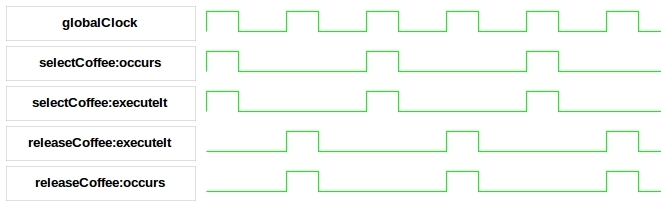
\includegraphics[width=.9\textwidth]{bcool/figs/runningeventvar}
			\caption{Resulting coordination of the Coffee Machine by using the global event variable globalClock}
			\label{fig:runningeventvar}
		\end{figure}



In this subsection, we have presented the abstract syntax of \bcool by relying on the running example operator. To specify this example, we used event expressions and relations that are defined in the library \emph{facilities.moccml} (Listing~\ref{lst:bcoolrunningexampletimed}: line 2). In \bcool, expressions and relations are defined in dedicated libraries that must be imported (\emph{ImportedLibStatement} in Figure~\ref{fig:bcool}). We introduce the notion of library in the following subsection.
	
	
	
%This subsection presents the syntactic elements of \bcool. The abstract syntax of \bcool is defined by its metamodel (see Figure~\ref{fig:bcool}). The metamodel is a particular implementation of the framework for coordination pattern approaches presented in Chapter~\ref{ch:framework}.  
	
%The root element is a \emph{BCoolSpecification} that contains \emph{Operators}. Each operator refers to \dse to specify what event types it coordinates. To get the \dse, a \bcool specification imports language behavioral interfaces (\emph{importsInterfaceStatements}). The number of imported interfaces is related with the number of models that the specification accepts as input. Since the \bcool specification is applied at least between two models, it imports at least two interfaces. The same interface, however, can be imported several times. This allows the specification of the coordination between homogeneous languages.  

%Each operator refers at least two \dse. We decide this implementation from the experimentation. 
%In \bcool, operators are used to specify when and how the referred \dse must be coordinated. To do so, each operator contains a \emph{correspondence matching} and a \emph{coordination rule}. The former is used to select instance of \dse and the latter to express how the selected instances must be coordinated. 

%A correspondence matching relies on a \emph{Condition} that contains an OCL Boolean expression. To express the boolean expression, an integrator can navigate through the context of the \dse to query a specific syntactic element, \eg attribute \emph{name}. The boolean condition is thus used to compare the queried elements. It acts as a precondition for the coordination rule, \ie it is a predicate that defines when the coordination rule must be applied to the given instances of \dse.

%The coordination rule contains the specification of the ``glue'' that coordinates instances of \dse. To express the glue, the coordination rule contains an \emph{EventRelation} and some \emph{EventVariables} (\emph{localEventVariables}). Event relations are used to restrict the relative order of the occurrences of events used as parameters. Its actual parameters can be instances of \dse, some \emph{EventVariables} and/or constants (\eg integer constants). Event relations are defined into a library that the integrator must import (\emph{ImportLibStatement}). The library is defined by using \moccml~\cite{moccmlbib} (Model of Concurrency and Communication Language). The notion of library is discussed in Subsection~\ref{subsec:bcoollib}.



%To illustrate the syntactic elements previously presented, we used \bcool to develop the running example operator, which is defined between the TFSM and Activity languages. We defined a \bcool specification named \emph{TFSMAndActivity} (see Listing~\ref{lst:bcoolrunningexample}) and we imported the language behavioral interface of each language. To do so, we imported the \ecl specification of each language and we named them \emph{activity} and \emph{tfsm}. Also, we imported the \moccml library \emph{facilities.moccml} that provides the event relations that are used latter for the coordination rule. 

%To specify the operator, we have to compare and coordinate FSMEvents and Actions by relying on theirs name. We specify so by defining an operator named \emph{SyncFSMEventsAndActions} that refers to the \dse \emph{FSMEvent::occurs} and \emph{Action::executeIt} and we mapped them as \emph{FSMEvenOccurs} and \emph{ActionExecute} respectively. Then, to select pair of instances of these \dse, we query their context to get the attribute \emph{name}. The attributes are used as operands for a boolean condition. When an instance of \dse \emph{occurs} and an instance of \dse \emph{executeIt} have the same name, the pairs are selected and the coordination rule is applied. To express a strong synchronization between the selected instances, we use the event relation \emph{Rendezvous}. This event relation accepts two events as arguments and forces the occurrences of these events to happen simultaneously. This relation is defined into the library.  



%The specification previously presented can be used to coordinate any pair of TFSM and Activity. In particular, we use it to coordinate the tfsm \emph{CoffeeCoin} and the activity \emph{CoffeeAlgorithm}. Figure~\ref{fig:runningrdv} shows the resulting coordination between the \mse \emph{selectCoffee:occurs} and \emph{selectCoffee:executeIt} in which the occurrences of these events happen simultaneously.  

%To support more complex coordination rules, \bcool enables the definition of new events by using \emph{EventVariables}. Such events can be either defined globally for the whole specification (\emph{globalEventVariables}) or locally within a coordination rule (\emph{localEventVariables}). When globally defined, event variables can be used to define global events used across different operators as synchronization variables. Local event variables, however, can be used in the coordination rule to create a new event from the selected instances of \dse and possibly from attributes of the input models. Then, they can be used as parameters of event relations, constraining by transitivity (some of) the occurrences of \dse instances. 

%Event variables can be initialized by using an \emph{EventExpression}. An event expression returns a new event from given parameters, which can be instances of \dse, some EventVariable and/or constants (\eg integer constants). For instance, an event expression can be used to filter the occurrences of a \dse instance, also, they can also be used to join in a single event the occurrences of different events (union). Event expressions are defined into a \moccml library that must be imported.   

%To illustrate the use of event variables, we modify the running example operator by considering the case in which the coordination between FSMEvents and Actions relies on a global clock signal. This situation is often in synchronous digital systems where a clock signal is used to coordinate the actions in a circuit. In this case, instances of FSMEvents and executeIt are still strongly synchronized, however, such synchronization happens only when a global clock ticks. To specify this in \bcool, we first define a global event variable named \emph{globalClock} (Listing~\ref{lst:bcoolrunningexampletimed}: line 5). Then, in the coordination rule, we use the globalClock together with the \dse \emph{occurs} and \emph{executeIt} to create two local event variables named \emph{sampledExecuteIt} and \emph{sampledOccurs} (Listing~\ref{lst:bcoolrunningexampletimed}: line 9 and 10). To initialize these local variables, we use the event expression \emph{SampleOn}. This expression accepts two events as parameters: the \emph{SampledEvent} and the \emph{Trigger}. \todo{The expression creates a new event by sampling the \emph{SampledEvent} with the \emph{Trigger} event. Then, in the coordination rule, we coordinate the resulting local events by a Rendezvous. However, such a coordination can be gather for future implementation by relying on a library. We the library notion in the following.}


    


	%\item  For example, in some cases only some occurrences of the selected events may be synchronized. Also, it may happen that the coordination relies on a global clock. 
	
	%\item This situation is often in synchronous digital systems where a clock signal is used to coordinate the actions in a circuit. In these cases, it would be necessary to do something on the selected instances of \dse before to apply the event relation. 
	
 

%	\item These variables either define global events used across different operators, or create a new event from the selected instances of \dse and possibly from attributes of the input models. 
	
	
	
	%\item  For instance, an event expression can be used to filter the occurrences of a \dse instance. An event expression can also be used to join in a single event the occurrences of different events (union). 
	
	%\item When used in the coordination rule, the resulting events can be used as parameters of event relations, constraining by transitivity (some of) the occurrences of \dse instances. Event expressions are also defined into \moccml libraries that must be imported. 
	
	
	%\item We illustrate the use of event variables by modifying the previous example. In this case, the synchronization of FSMEvents and Actions is based on a global clock signal. The coordination happens only when the global clock ticks. To do so, we need to define a global event variable that act as global clock, and then, modify the coordination rule. 
	
	%\item First, we define a global event variable named \emph{globalClock}(Listing~\ref{lst:bcoolrunningexampletimed}: line 5). Then, in the coordination rule, we use the globalClock together with the \dse \emph{occurs} and \emph{executeIt} to create two local event variables named \emph{sampledExecuteIt} and \emph{sampledOccurs} (Listing~\ref{lst:bcoolrunningexampletimed}: line 9 and 10). To initialize them, we rely on the event expression \emph{Sample}. 
	
	%\item TODO: What does sample do? 
	
	%\item How local events are syncronized 
	
	%\item However, such a coordination can be gather for future implementation by relying on a library. We the library notion in the following.
	
	%\item The resulting events tick if and only if the global clock and the instance of \dse have also ticked. For instance, the event \emph{sampledOccurs} only ticks if globalClock and the instance of \dse \emph{occurs} ticks. In this case, we use a global event variable together with event expressions to sample the occurrences of selected instances of \dse. Then, we can use the local events as parameters of event relations, constraining by transitivity (some of) the occurrences of \dse instances. In our example, we force a simultaneous occurrence between the local events by using the relation rendezvous (Listing~\ref{lst:bcoolrunningexample2}: line 13). As a result, instances of \dse occurs and startAction happen simultaneously (see Figure~\ref{fig:runningeventvar}). 



%The main element of \bcool (see Figure~\ref{fig:bcool}) is a \emph{BCoolSpecification} that contains language behavioral interfaces (\emph{importsInterfaceStatements}) and \emph{Operators}. The specification must import at least two language behavioral interfaces. Interfaces provide the \emph{DSE} needed for the coordination. The imported \dse serve as parameters for the operators. Then, an operator specifies what instances of these \dse are selected and how they are coordinated (the \emph{DSEs} reference). For instance, to build the running example, we synchronize FSMEvents and the starting of Actions. This is done by coordinating the instances of \dse \emph{occurs} and \emph{startAction} (see Appendix~\ref{ap:languages}). To do so, in a \bcool specification named \emph{SyncFSMEventsAndActions} (Listing~\ref{lst:bcoolrunningexample}: line 1), we import the language behavioral interface of TFSM and Activity (Listing~\ref{lst:bcoolrunningexample}: line 3 and 4). Then, we define the operator named \emph{SyncProduct} with \emph{occurs} and \emph{startAction} as parameters  (Listing~\ref{lst:bcoolrunningexample}: line 6). 

%Each operator contains both a \emph{correspondenceMatching} and a \emph{coordinationRule}. The former relies on a Boolean \emph{Condition} defined as an OCL expression. It acts as a precondition for the coordination rule, \ie it is a predicate that defines when the coordination rule must be applied to the given parameters. To specify the predicate, it is possible to navigate through the context of the \dse and query a specific element used within the Boolean expression. For instance, for the running example, the condition selects pairs of instance of \dse \emph{occurs} and \emph{startAction} by looking at its attribute \emph{name} (Listing~\ref{lst:bcoolrunningexample}: line 7). %This corresponds with a correspondence that relies on a naming convention. We call such a correspondence implicit, however the correspondence may be explicit, we study that case in Section~\ref{subsubsec:explicitcorrespondence}.

%The \emph{coordinationRule} specifies how the selected instances of \dse must be coordinated. To do so, the user must define \emph{EventRelation} and some \emph{EventVariables} (\emph{localEventVariables}).

%Event relations restrict the occurrences of the events on which it is applied. The actual parameters of the event relation can be some instances of \dse and/or some \emph{EventVariables}. For instance, in the running example we want a strong synchronization between FSMEvents and Actions. Thus, the coordination rule uses a ``rendez-vous'' relation between the selected instances of \dse \emph{occurs} and \emph{startAction} (see Appendix~\ref{ap:expressionandrelations}). As a result, all the occurrences of these events are forced to happen simultaneously. Figure~\ref{fig:runningrdv} shows the resulting coordination in the case of the coffee machine. The instance of \dse \emph{occurs} and \emph{startAction} happens simultaneously.

%Lots of other relations, more or less complex can be defined, \eg \emph{Causality}, \emph{FIFO} or ad-hoc relations for specific protocols. For instance, Figure~\ref{fig:runningrunningcausality} illustrates the resulting coordination if we use the event relation \emph{Causality}. The definition of event relations is made in dedicated libraries, which must be imported (see Section~\ref{subsec:bcoollib}).
